\newpage
\graphicspath{{../choicungbi/tangram/}}
\blfootnote{$^1$Công ty Cổ phần phát triển giáo dục POMATH.}
	\begingroup
	\AddToShipoutPicture*{\put(42,595){\includegraphics[scale=0.7]{../tangram/toancuaBi_2-tieude}}} % %Image background
	\centering
	\endgroup	
	
\vspace*{25pt}

	Mở đầu cho bài viết trong số này, Bi xin mời các bạn quan sát các hình ảnh sau:
	\begin{figure}[H]
		\vspace*{-5pt}
		\centering
		\captionsetup{labelformat=empty}
		\begin{subfigure}{.45\textwidth}
		\captionsetup{labelformat=empty}
		\centering
		
\includegraphics[width=.5\linewidth]{image1}
		\caption{\small \it Hình $1$}
		\end{subfigure}
		\begin{subfigure}{.45\textwidth}
		\captionsetup{labelformat=empty}
		\centering
		
\includegraphics[width=.5\linewidth]{image2}
		\caption{\small \it Hình $2$}
	\end{subfigure}
	\vspace*{-10pt}
\end{figure}	
	Các bạn tưởng tượng ra hình gì?
	\vskip 0.1cm
	Chắc là các bạn sẽ tưởng tượng ra hình trái tim, hình con thuyền, cũng có bạn lại nghĩ đây là hình con chim. Nhưng các bạn có tìm ra được đặc điểm chung của hai hình trên không?
	\begin{multicols}{2}
		Bi xin bật mí với các bạn, hai hình này có cùng diện tích đấy! Hay chính xác hơn, cả hai hình này đều được ghép từ $7$ mảnh ghép. Xem này:
		\begin{figure}[H]
			\vspace*{5pt}
			\centering
			\captionsetup{labelformat=empty}
			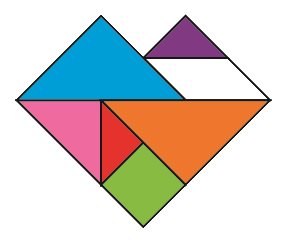
\includegraphics[width=.4\linewidth]{imame3}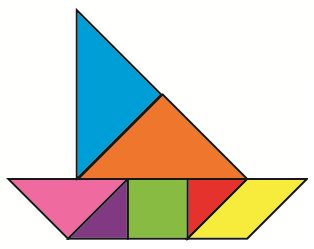
\includegraphics[width=.4\linewidth]{image4}
			\caption{\small \it Hình $3$\hspace*{30pt} Hình $4$}
			\vspace*{-10pt}
		\end{figure}
	\end{multicols}
	Nếu bạn nào còn băn khoăn vì sao hai hình khác nhau nhiều như thế mà diện tích lại bằng nhau thì Bi xin mời các bạn xem tiếp $7$ mảnh ghép này Biến hóa như thế nào nhé!
	\begin{multicols}{2}
		Đến bây giờ thì các bạn đều hiểu rồi chứ? Chúng ta đều có thể cắt ghép hai hình ban đầu thành $7$ mảnh ghép, rồi dùng $7$ mảnh ghép đó ghép lại thành một hình vuông. Vì vậy, chúng có diện tích bằng nhau. Quả là rất thú vị phải không?
		\begin{figure}[H]
			\vspace*{5pt}	
			\captionsetup{labelformat=empty}
			\centering
			\captionsetup{justification=raggedleft}
			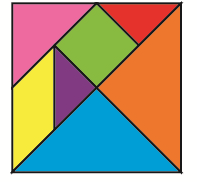
\includegraphics[width =0.3\textwidth]{image5}
			\caption{\small\it Hình $5$.}
			\vspace*{-10pt}
		\end{figure}
	\end{multicols}
	Và các bạn Biết không, những gì Bi vừa giới thiệu trên đây đều xuất phát từ một trò chơi mang tên gọi: TANGRAM.
	
	\vspace*{-5pt}
	\begin{multicols}{2}
		Tangram là một món đồ chơi xuất hiện rất lâu đời ở Trung Quốc. Theo tiếng Trung Quốc, ``Tangram" nghĩa là ``$7$ mảnh ghép thông minh", gồm $7$ mảnh ghép (Gọi là ``tans") được cắt ra từ một hình vuông lớn, bao gồm: $1$ hình vuông, $1$ hình bình hành, $2$ tam giác vuông cân nhỏ, $1$ tam giác vuông cân vừa và $2$ tam giác vuông cân lớn.
		\vskip 0.1cm
		\textit{\small (Tam giác vuông cân là tam giác có một góc vuông và có $2$ cạnh bằng nhau)}
		\begin{figure}[H]
			\vspace*{-20pt}	
			\captionsetup{labelformat=empty}
			\centering
			\captionsetup{justification=raggedleft}
			
\includegraphics[width =0.2\textwidth]{image6}
			\caption{\small\it Hình $6$.}
%			\vspace*{5pt}
		\end{figure}
	\end{multicols}
	\vspace*{-5pt}
	Luật chơi của Tangram rất đơn giản: Dùng đúng $7$ mảnh ghép của trò chơi để xếp ra các hình có nghĩa khác nhau, đảm bảo các mảnh ghép không trùng lên nhau.
	\vspace*{-5pt}
	\begin{multicols}{2}
		\begin{figure}[H]
			\vspace*{5pt}	
			\captionsetup{labelformat=empty}
			\centering
			\captionsetup{justification=raggedleft}
			
\includegraphics[width =0.2\textwidth]{image7}
			\caption{\small\it Hình $7$.}
			\vspace*{-10pt}
		\end{figure}
		Đầu thế kỉ $19$, Tangram đã vượt ra khỏi Biên giới Trung Quốc thông qua những con tàu buôn của những nhà thương gia phương Tây. \linebreak Tangram đặt chân đến Mỹ, các nước Châu Âu và nhanh chóng tạo ra cơn sốt về một trò chơi thú vị nhưng cũng đầy thách thức. Cũng từ đó, Biến thể của
		Tangram xuất hiện ngày càng nhiều, không còn giữ nguyên khuôn hình vuông như ban đầu nữa. Vì vậy, số lượng hình ghép được tăng lên gấp nhiều lần và đương nhiên, những hình ``cực khó" cũng xuất hiện với mật độ ngày càng lớn.
		\begin{figure}[H]
			\vspace*{-10pt}	
			\captionsetup{labelformat=empty}
			\centering
			\captionsetup{justification=raggedleft}
			
\includegraphics[width =0.2\textwidth]{image8}
			\caption{\small\it Hình $8$.}
%			\vspace*{-10pt}
		\end{figure}
		Nhìn các hình ảnh trên, các bạn đã thấy hấp dẫn chưa? Nhưng điều hấp dẫn hơn sẽ nằm ngay sau đây: Bi sẽ hướng dẫn các bạn tự tạo ra bộ trò chơi này mà không cần đi mua ở đâu cả. Chúng ta bắt đầu nhé!
	\vskip 0.1cm
	\textbf{Chuẩn bị và thực hiện}
	\vskip 0.1cm
	\textbf{* Chuẩn bị:}
	\vskip 0.1cm
	-- $1$ tờ giấy bìa hình vuông kích thước $8$cm $\times$ $8$cm.
	\vskip 0.1cm
	-- Thước kẻ, bút chì, kéo, màu sáp.
	\vskip 0.1cm
	\textbf{* Thực hiện:}
	\vskip 0.1cm
	\textit{Bước $1$:} Kí hiệu tờ bìa hình vuông là $ABCD$ (hình vẽ).
	\vskip 0.1cm
	\textit{Bước $2$:} 
	\vskip0.05cm
	+/ Trên cạnh $AB$ lấy điểm $E$ sao cho $AE = EB = 4cm$.
	\vskip 0.1cm
	+/ Trên cạnh $AD$ lấy điểm $F$ sao cho $AF = FD = 4cm$.
	\vskip 0.1cm
	+/ Trên đoạn $EF$ lấy điểm $G$ sao cho $GE= GF$.
	\vskip 0.1cm
	+ Trên đoạn $BD$ lấy các điểm $H, O, I$ sao cho $DH = HO = OI = IB$.
	\vskip 0.1cm
	\textit{Bước $3$:} Nối $G$ với $O, G$ với $H, O$ với $C, E$ với $I$.
	\begin{figure}[H]
		\vspace*{-10pt}
		\centering
		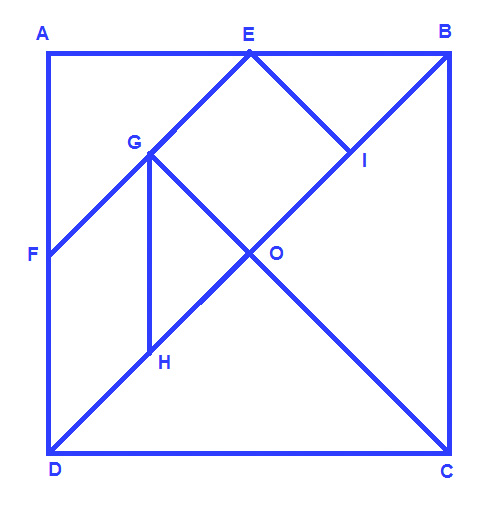
\includegraphics[scale=0.2]{image9}
		\vspace*{-10pt}
	\end{figure}
	\textit{Bước $4$:} Dùng kéo cắt thành $7$ mảnh rồi dùng màu sáp tô màu theo ý thích.
	\end{multicols}
	Chúng ta đã tạo ra được một bộ Tangram rồi, thật là dễ đúng không? Các bạn hãy dùng bộ Tangram vừa tạo để ghép các hình phía trên nhé!
	\vskip 0.1cm
	Nhưng Bi luôn có một câu hỏi: ``Liệu chúng ta có thể tự tạo ra cho mình một bộ Tangram?". Không Biết có bạn nhỏ nào cũng đặt câu hỏi giống như Bi không?
	\vskip 0.1cm
	Vậy thì chúng ta thử cùng nhau nghiên cứu các bộ Tangram xem phát hiện ra được điều lí thú gì nhé!
	\begin{figure}[H]
	\centering
	\vspace*{-10pt}
	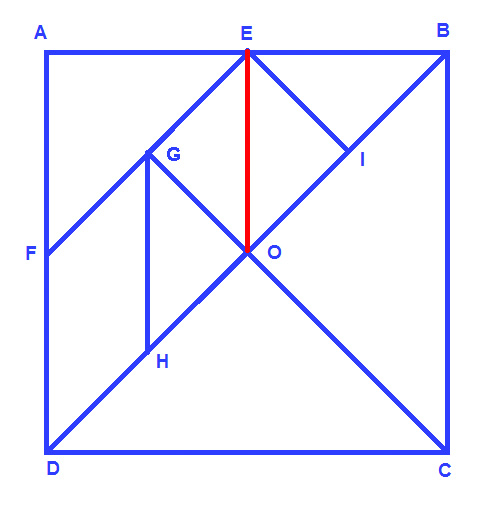
\includegraphics[scale=0.2]{image10}\quad
	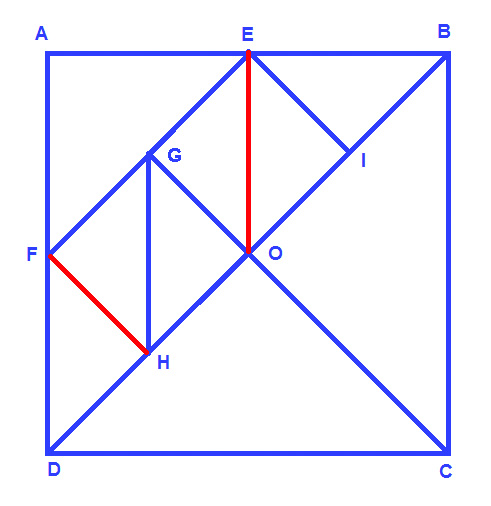
\includegraphics[scale=0.2]{image11}\quad
	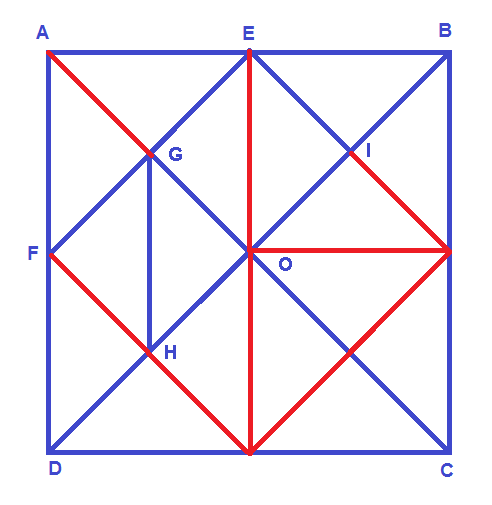
\includegraphics[scale=0.2]{image12}
	\end{figure}
	\textit{Bi nhận thấy, hình vuông $OIEG$ có thể chia thành $2$ tam giác vuông nhỏ. Lúc này, ta có $2$ hình  bình hành bằng nhau là $DHGF$ và $HOEG$}
	\vskip 0.1cm
	\textit{Vì vậy, hình bình hành $DHGF$ cũng có thể chia thành $2$ tam giác vuông nhỏ như hình bình hành $HOEG$.
	\vskip 0.1cm
	Liệu các mảnh còn lại có chia được thành các tam giác vuông nhỏ như trên?}
	\vskip 0.1cm
	\textit{Câu trả lời là có.
	\vskip 0.1cm
	Tất cả $7$ mảnh của bộ Tangram này đều được tạo ra từ $1$ hay nhiều tam giác vuông cân cùng kích thước.}
	\begin{multicols}{2}
	Quả là bất ngờ đúng không các bạn? Như vậy, chúng ta chỉ cần sử dụng các tam giác vuông cân giống nhau là có thể tạo ra một bộ Tangram mới rồi! Ví dụ, Bi sẽ chọn cách ghép các tam giác vuông như sau:
	\vskip 0.1cm
		Bây giờ, các bạn hãy tạo một bộ Tangram giống của Bi và ghép thành các hình sau. Đừng quên tưởng tượng xem mỗi hình ảnh thể hiện sự vật gì nhé!
		\begin{figure}[H]
			\vspace*{-15pt}
			\centering
			\captionsetup{labelformat=empty}
			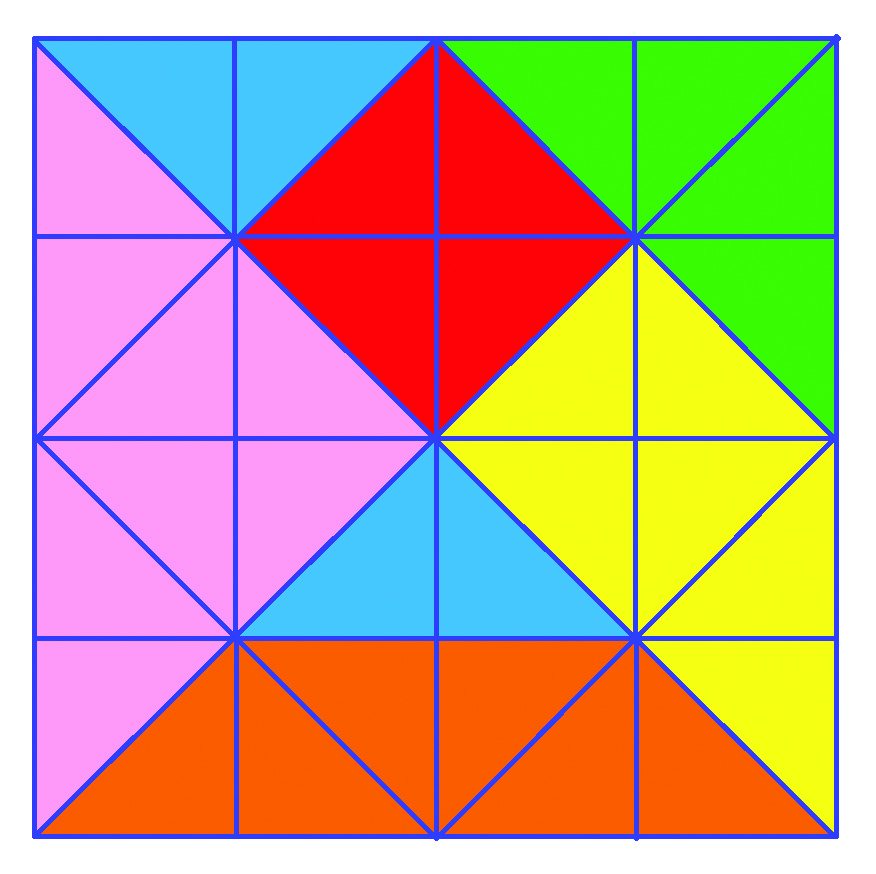
\includegraphics[width=0.25\textwidth]{image13}
			\caption{\small \it Hình $9$ -- Bộ Tangram gồm $4$ tam giác vuông cân, $1$ hình vuông, $1$ hình thang vuông, $1$ hình thang cân}
			\vspace*{-5pt}
		\end{figure}
	\end{multicols}
	\begin{figure}[H]
		\vspace*{-5pt}
		\centering
		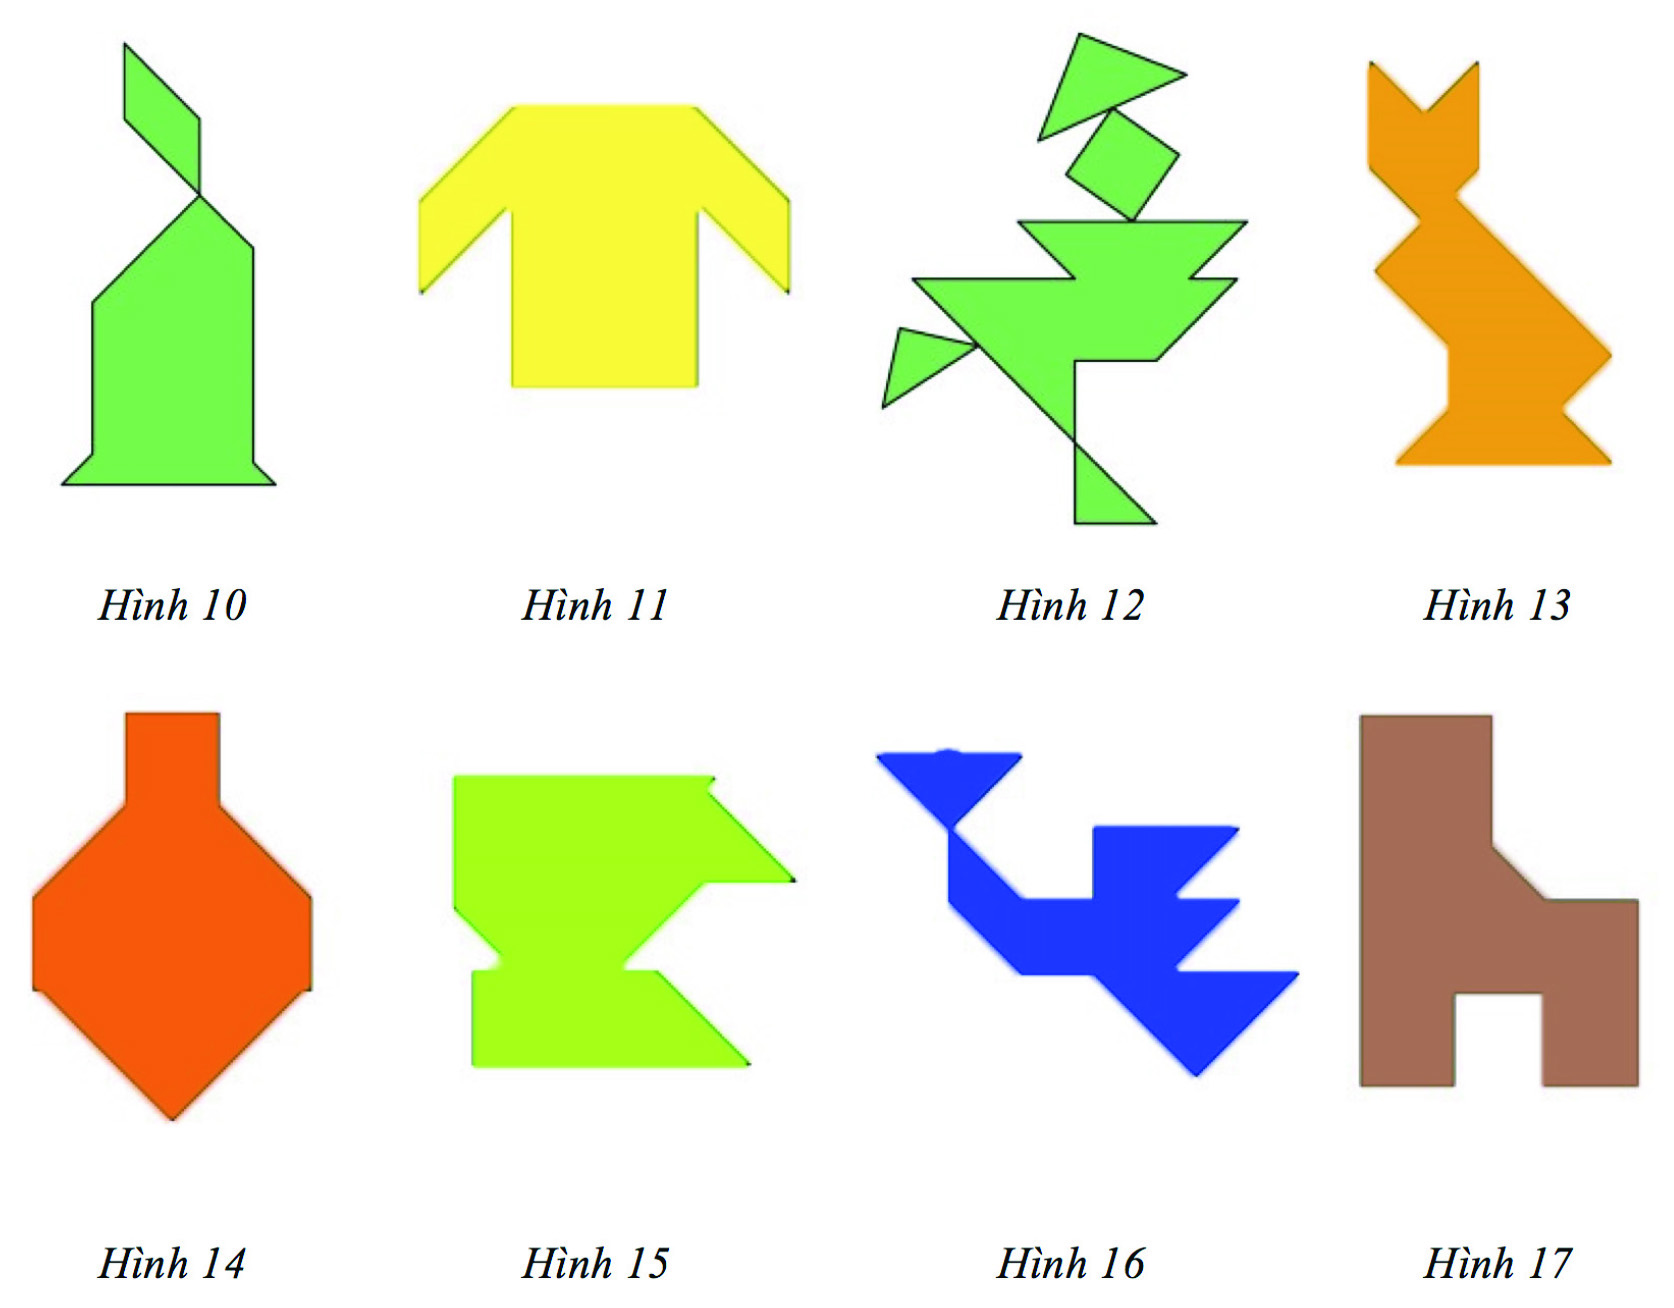
\includegraphics[width=0.65\textwidth]{cat-10}
		\vspace*{-5pt}
	\end{figure}


